\begin{figure}[h!]
    \centering
    \resizebox{\columnwidth}{!}{
    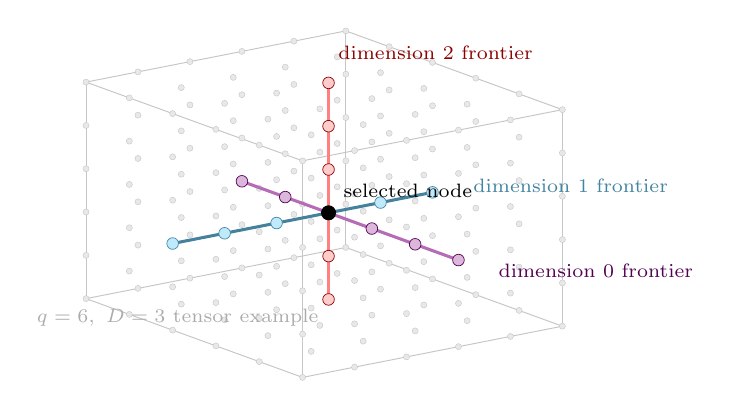
\begin{tikzpicture}[
        x={(0.55cm,-0.20cm)},
        y={(0.66cm,0.13cm)},
        z={(0cm,0.55cm)},
        every node/.style={font=\scriptsize},
        cube edge/.style={gray!45,line width=0.35pt},
        base dot/.style={circle,draw=gray!45,fill=gray!18,line width=0.15pt,minimum size=2.2pt,inner sep=0pt},
        purple dot/.style={circle,draw=violet!65!black,fill=violet!28,line width=0.25pt,minimum size=4.2pt,inner sep=0pt},
        blue dot/.style={circle,draw=cyan!60!black,fill=cyan!25,line width=0.25pt,minimum size=4.2pt,inner sep=0pt},
        red dot/.style={circle,draw=red!55!black,fill=red!20,line width=0.25pt,minimum size=4.2pt,inner sep=0pt},
        selected dot/.style={circle,draw=black,fill=black,minimum size=5pt,inner sep=0pt},
        purple line/.style={violet!58,line width=1.1pt},
        blue line/.style={cyan!58!black,line width=1.1pt},
        red line/.style={red!50,line width=1.1pt}
    ]
        \def\sx{2}
        \def\sy{3}
        \def\sz{2}

        \draw[cube edge] (0,0,0) -- (5,0,0) -- (5,5,0) -- (0,5,0) -- cycle;
        \draw[cube edge] (0,0,5) -- (5,0,5) -- (5,5,5) -- (0,5,5) -- cycle;
        \draw[cube edge] (0,0,0) -- (0,0,5);
        \draw[cube edge] (5,0,0) -- (5,0,5);
        \draw[cube edge] (5,5,0) -- (5,5,5);
        \draw[cube edge] (0,5,0) -- (0,5,5);

        \foreach \x in {0,...,5} {
            \foreach \y in {0,...,5} {
                \foreach \z in {0,...,5} {
                    \node[base dot] at (\x,\y,\z) {};
                }
            }
        }

        \draw[purple line] (0,\sy,\sz) -- (5,\sy,\sz);
        \draw[blue line] (\sx,0,\sz) -- (\sx,5,\sz);
        \draw[red line] (\sx,\sy,0) -- (\sx,\sy,5);

        \foreach \x in {0,...,5} {
            \node[purple dot] at (\x,\sy,\sz) {};
        }
        \foreach \y in {0,...,5} {
            \node[blue dot] at (\sx,\y,\sz) {};
        }
        \foreach \z in {0,...,5} {
            \node[red dot] at (\sx,\sy,\z) {};
        }
        \node[selected dot,label={[font=\scriptsize]above right:selected node}] at (\sx,\sy,\sz) {};

        \node[text=violet!65!black,anchor=west] at (5.7,\sy,\sz) {dimension 0 frontier};
        \node[text=cyan!60!black,anchor=west] at (\sx,5.6,\sz) {dimension 1 frontier};
        \node[text=red!55!black,anchor=west] at (\sx,\sy,5.7) {dimension 2 frontier};
        \node[anchor=west,text=gray!65] at (-0.4,-0.8,-0.4) {\(q=6,\ D=3\) tensor example};
    \end{tikzpicture}
    }
    \caption{Tensor quorum geometry for \(q=6\) and \(D=3\). The selected node is placed in a \(6 \times 6 \times 6\) coordinate tensor. Each pastel line fixes the selected node's coordinates in all but one dimension; the free dimension is one future quorum frontier. In v2, prefill dispatch sends the local block to the union of these future contacts before verified consensus skips the old first data-spreading round.}
    \label{fig:tensor_prefill_cube}
\end{figure}
